\chapter{人工智能模型初探（周子祺）}
在本章中，我们将带领读者动手体验人工智能模型，让读者对其有一个基本的感知。本章从简要回顾人工智能基础任务开始，介绍在不同任务下人工智能模型的选择，让读者对模型的多样性和适用性有一个宏观的认识。然后我们将以一个可视化项目为例，向大家简单介绍如何通过动手调试关键参数，模拟不同的训练过程，以实现我们期望的结果。在这个过程中，我们会向读者详细介绍人工智能模型中一些常用的超参数，模拟模型训练的过程，展示这些超参数如何影响模型的性能和结果，引领读者感知参数调整的重要。

\section{模型的选择}

在本节中，我们将回顾前面所探讨的人工智能的基本任务，包括学习、预测、分类与回归以及生成与优化等。我们以线性回归和逻辑回归任务为例，向读者介绍两种回归任务的历史以及实际应用场景，并分析它们在解决相关问题时的优势和局限性。这将帮助读者更加深入地理解不同人工智能模型的特点，以及如何根据任务需求选择合适的模型。

\subsubsection{1、线性回归} 
\setlength{\parindent}{2em}
\begin{itemize}
    \item \textbf{定义与历史:} 
             \setlength{\parindent}{2em}
       
线性回归是机器学习中最基础的建模方法之一，其核心在于探索自变量与因变量之间的线性关系。通过构建数学模型，线性回归可以帮助我们理解变量之间的关系，并对未知的数据进行预测。
    
线性回归的历史可以追溯到19世纪初，1855年，英国统计学家弗朗西斯·高尔顿在研究人类身高遗传问题时，提出了“回归到平均值”的概念，这便是线性回归名称的由来。随着时间的推移，线性回归经过不断发展和改进，研究人员提出了各种改进的线性回归模型，如多元线性回归、岭回归（Ridge Regression）、Lasso回归等。近年来，随着人工智能的兴起，线性回归算法被运用到一些更复杂的模型中，如神经网络中的线性层、决策树和随机森林、梯度向量机等。当前，线性回归已经成为一种广泛应用的预测和分析工具，在人工智能、统计等领域中扮演着重要的角色。

\begin{figure}[ht]
  \centering
  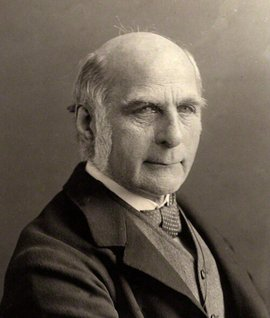
\includegraphics[width=0.6\linewidth]{image/5/1.jpg}
  \caption{弗朗西斯·高尔顿图片(待优化)}
  \label{fig:my_label}
\end{figure}

\item \textbf{优势分析：}
         \setlength{\parindent}{2em}

简单易懂：线性回归模型是一个简单而直观的模型，便于读者理解。
        
计算效率高：训练线性回归模型的计算效率通常较高，尤其是在大规模数据集上。
        
可解释性：线性回归模型提供了自变量与因变量之间的线性关系，模型的系数可以解释为变量对因变量的影响程度。

灵活性：线性回归模型可以扩展到多种模型上，成为它们构建的基础。同时，线性回归模型也可以运用到金融、社会学、人工智能等领域中。


\item \textbf {局限性探讨：}
        \setlength{\parindent}{2em}
    
非线性关系拟合不足：线性回归对非线性关系的数据模式表现不佳，例如二次关系、指数关系、余弦关系等。

对异常值敏感：线性回归对异常值（离群点）敏感，这可能导致模型的不稳定性。

多重共线性问题：当自变量之间存在高度相关性时，可能导致回归系数的估计不准确。

    \item \textbf {实际应用：}
            \setlength{\parindent}{2em}
        
在详细分析了线性回归模型的优点和局限性之后，我们可以更进一步探讨它在实际应用中的作用。由于线性回归模型简单易懂、计算效率高，并且具有良好的可解释性，这些特点使得它特别适合完成两项任务：预测未来会发生什么，以及优化我们对数据的理解和拟合。简而言之，线性回归模型在预测和优化这两大领域发挥了重要的作用，接下来，我们具体探讨一下它分别在预测和优化任务中的实际应用。
        
预测任务：在预测任务中，线性回归是一种强大的工具，它能够基于一个或多个自变量来预测连续的因变量。例如，研究者通过建立线性回归模型，利用固定资产投资、社会消费品总额、净出口等自变量来评估这些经济指标对GDP增长的影响，并成功预测了中国的GDP增长率。此外，线性回归模型还被广泛应用于商业营销与商品定价、金融分析、疾病预防等多个行业领域。

优化任务：在优化任务中，线性回归模型的应用同样广泛，它可以帮助我们找到最优的参数组合。在相关研究中，研究者们开发了一个模型来预测风速，在这一模型架构中，线性回归模型被用于处理神经网络产生的预测结果与误差序列，进而优化模型的预测精度，并增强整体模型的稳定性。这有效平衡了发电成本与效率，还提升了电网稳定性及可再生能源的利用效率。此外，线性回归的应用展示了其在资源分配、能源消耗最小化、生产效率提升等多个领域中的重要价值，显示出它在优化任务中的重要价值。
\end{itemize}
\subsubsection{2、逻辑回归}
% \setlength{\parindent}{2em}
\begin{itemize}

    \item \textbf{定义与历史:} 
           \setlength{\parindent}{2em}

逻辑回归是机器学习和统计学中的一种关键建模技术，其核心在于分析一个或多个自变量与一个二元因变量之间的逻辑关系。通过建立数学模型，逻辑回归能够预测数据属于某个类别的概率，广泛应用于分类问题。
          
逻辑回归的历史起源于19世纪，由比利时数学家皮埃尔-弗朗索瓦·韦尔胡斯特提出，用于描述人口增长的逻辑曲线。20世纪初，该模型被引入生物测定领域，用于研究药物剂量与生物效应的关系。1944年，Joseph Berkson首次提出“逻辑回归”这一术语，并推广了其在统计学中的应用。随着计算机技术的发展，逻辑回归因其在处理二元结果数据方面的优势而被广泛应用于医学、流行病学和社会科学等多个领域。逻辑回归模型的多变量和多类别扩展进一步增强了其在数据分析中的实用性，使其成为当今机器学习和数据科学中不可或缺的预测和分类工具。

        
    \item \textbf{优势分析:} 
           \setlength{\parindent}{2em}

简单易懂： 逻辑回归模型相对简单，易于理解和解释，特别是模型的系数可以解释为特征对于事件发生概率的影响。
            
适用于二元结果分析：逻辑回归特别适用于分析二元结果，使得它在医学、流行病学和社会科学研究中非常有用。

灵活性：逻辑回归模型可以处理多个自变量，包括连续和分类变量，这使得它在多变量分析中非常灵活。

参数估计的稳健性：逻辑回归使用最大似然估计，这是一种广泛认可的参数估计方法。
           
\item \textbf{局限性探讨:} 
    
           \setlength{\parindent}{2em}
分类变量的限制：对于分类变量，逻辑回归需要使用设计变量（dummy variables），这可能会增加模型的复杂性，尤其是在处理多个类别的分类变量时。
        
模型不稳定性：当样本量较小或结果变量的事件发生率接近0或1时，模型的估计可能会变得不稳定。
        
异常值的敏感性：逻辑回归对异常值比较敏感，异常值可能会影响模型的参数估计。

    \item \textbf{实际应用:} 
           \setlength{\parindent}{2em}
           
在深入探讨了逻辑回归模型的优势和局限性之后，我们能够更进一步理解它在实际应用中的重要性。逻辑回归模型因其简单易懂、适用于二元结果分析，以及在多变量分析中的灵活性和参数估计的稳健性，这些特点使得它特别适合完成三项关键任务：预测特定事件发生的概率，对事物类别的分类以及对数据的优化。接下来，我们具体探讨一下它的实际应用。
            
预测任务：逻辑回归同样适用于预测任务中。例如，研究者利用逻辑回归对亚马逊的客户评论进行情感分析，以评估消费者对产品的态度。除了情感分析，逻辑回归还可以用来预测疾病。逻辑回归模型被应用于构建一个糖尿病风险评估体系，以预测个体是否可能患有糖尿病。除此之外，逻辑回归在金融风险分析、股票预测等领域也发挥着重要的作用。
            
分类任务：逻辑回归也应用在分类任务中。研究者利用逻辑回归模型对MNIST数据集中的手写数字图像进行分类，以评估模型对图像中数字的识别能力，这表明了逻辑回归在计算机视觉领域的应用价值。同时，在医疗领域，特别是在基因表达数据分析中，逻辑回归也被用于分类不同疾病状态下的样本。这种应用展示了逻辑回归在生物信息学和精准医疗中的重要性。
            
优化任务：逻辑回归在优化任务中也有应用。例如，逻辑回归可以用来优化资源分配以及定价策略。
\end{itemize}

\section{模型配置介绍与优化} 

在本节中，我们将深入探讨人工智能模型中部分关键超参数的普适性概念，这些超参数对于模型的学习过程和最终性能至关重要。我们将详细解释每个超参数的作用、它们如何影响模型的训练动态，以及如何根据具体的应用场景进行调整，以实现最优的模型性能。我们将以烹饪慕斯蛋糕的艺术来比喻模型中超参数，揭示这些参数是如何影响模型的“烘焙”过程和蛋糕最终的“美味”程度。

\subsubsection{1、特征（Features）}

制作慕斯蛋糕首先需要我们挑选优质的原料，比如新鲜的牛奶、玉米淀粉、鸡蛋黄等。原材料的质量能够直接影响到慕斯蛋糕最终的口感和质地。在模型训练中，特征就像是这些原材料，它是指那些被用来预测或分类的输入变量。“精心挑选”的特征可以帮助我们更好地捕捉那些隐藏在数据中的信息，让训练的模型更加精准，就如同选择正确且优质的原料对蛋糕的口味至关重要一样。

\subsubsection{2、批量大小（Batch Size）}

制作慕斯蛋糕的第一步是制作慕斯糊，而批量大小类似于每次搅拌慕斯糊的量。搅拌的量太少，原料可能无法充分混合，导致蛋糕的口感不均匀；一次性搅拌的量过多，则可能使慕斯糊中的气泡消失或者凝聚成大气泡，导致慕斯过于紧实，而失去轻盈润滑的口感。在模型训练中，批量大小代表着每次训练更新时所使用的数据量，影响着内存的使用和训练的效率。因此，选择合适的批量大小是至关重要的，不仅需要在确保模型能够进行有效学习的同时，也要考虑到计算资源的限制，以达到最佳的训练效果。

\subsubsection{3、学习率（Learning Rate）}

在烘焙慕斯蛋糕的过程中，糖的分量对慕斯蛋糕的味道至关重要。如果糖放得过多，蛋糕可能会过甜，掩盖了其他原料的风味；而糖放得过少，则可能导致蛋糕不够入味，无法满足顾客的口味。类似地，在模型训练中，学习率是梯度下降算法中用于调整参数更新步长的超参数。它决定了在每次迭代中，模型参数更新的幅度。过大的学习率可能会导致模型训练不稳定，难以收敛；而太小的学习率则可能使模型训练过程过于缓慢，无法有效捕捉数据中的模式。因此，合理设置学习率对于训练出性能优异的模型至关重要。

\subsubsection{4、迭代次数（Epochs）}

烘焙时间是烹饪蛋糕的关键因素，决定了蛋糕的熟度和风味。如果烘焙时间不足，慕斯蛋糕可能会过于柔软，难以达到理想的质地和稳定性，从而影响其整体结构和口感；烘焙时间过长，可能会导致慕斯蛋糕的表皮干燥甚至会焦糊。在模型训练中，迭代次数决定了模型学习数据的完整遍数，也就是说，迭代一次意味着模型对每个样本都学习了一次。迭代次数过少，模型学习可能会不足，难以得到性能好的模型；次数过多，则可能会导致模型过拟合，即模型在训练数据上表现很好，但在新数据集上表现欠佳，难以应用在新的数据集上。

\subsubsection{5、正则化（Regularization）}

在慕斯蛋糕的配方中，除了主要的原料如牛奶、鸡蛋黄外，有时还会加入一些平衡剂，比如一小勺盐，以提升蛋糕整体的口感。在模型训练中，正则化的作用类似于这种平衡剂，它通过在损失函数里加上一点“盐”，也就是对模型参数的惩罚，防止模型过度拟合，帮助模型保持“健康”。让它在遇到新的数据时，能够更好地预测，而不是只记住训练数据，从而提高了模型的泛化能力。

\subsubsection{6、隐藏层（Hidden Layers）}

慕斯蛋糕的美味不仅仅来自于它的表层，而是每一层都为其最终的口感贡献了独特的风味，例如，表层有时会涂一层薄油以增加蛋糕表面的光泽和润滑度。慕斯层则是决定蛋糕的主要口味的关键。通过多层次的组合和相互作用，蛋糕拥有更好的口感。在模型训练中，隐藏层的作用就好比做慕斯蛋糕的中间层次，它是指介于输入层和输出层之间的层。通过提取输入数据的特征，并将这些特征的信息进行有效整合，从而提升模型的最终预测性能。

\subsubsection{7、噪声（Noise）}

在烘焙蛋糕的过程中，除了主要原料之外，还会有一些不纯物质或者意外的添加物，比如多余水分或杂质等，这会影响蛋糕入口的口感。类似地，在模型训练中，数据中的噪声就像是这些不期望的成分，它们是数据收集和处理过程中不可避免的一部分。噪声可能会干扰模型的学习过程，使得模型难以捕捉到数据中真正有用处的信息。因此，我们可能需要采取一些措施，比如滤波或异常值检测，来减少噪声的影响，帮助模型更准确地学习和预测。

\subsubsection{8、训练集和测试集比例（Training to Test Data Ratio）}

现在，我们成功制作出一批慕斯蛋糕，合理分配品尝测试的蛋糕比例显得十分重要，以确保对蛋糕的整体口味有一个准确的评估。正如同一道菜品在厨师和顾客口中可能有不同的评价，模型训练中训练集和测试集的比例同样至关重要。训练集用于构建模型，而测试集用于评估模型的性能。二者正确的比例可以确保模型在新数据上表现良好。

\subsubsection{9、损失函数（Loss Function）}

最后，味觉测试是检查蛋糕是否达到预期味道的最终步骤。每当我们从烤箱中取出制作好的蛋糕样本进行尝试时，我们都需要品尝它们是否达到了我们期望的味道。有的时候盐放多了，慕斯蛋糕的味道可能过重，我们就知道在下次烹饪时需要调整盐的分量。在模型训练中，损失函数的作用就像是一种“尝味”工具。它衡量模型的预测结果与实际结果之间的差距，如果模型的预测不准确，损失函数就会显示出一个较大的值，指导模型优化的方向，就像检查蛋糕的味道是否符合预期一样。

\section{模型参数调整与结果分析} 

在本节中，我们将结合实际案例，通过对比分析，直观展示不同参数设置下模型性能的变化，以及模型在训练集和测试集上的表现差异。此外，我们还会简单讨论参数调整过程中可能遇到的挑战，如过拟合、欠拟合问题等，并向大家介绍如何寻找模型的最优参数。

\subsubsection{1、总体介绍}
    
\begin{figure}[ht]
  \centering
  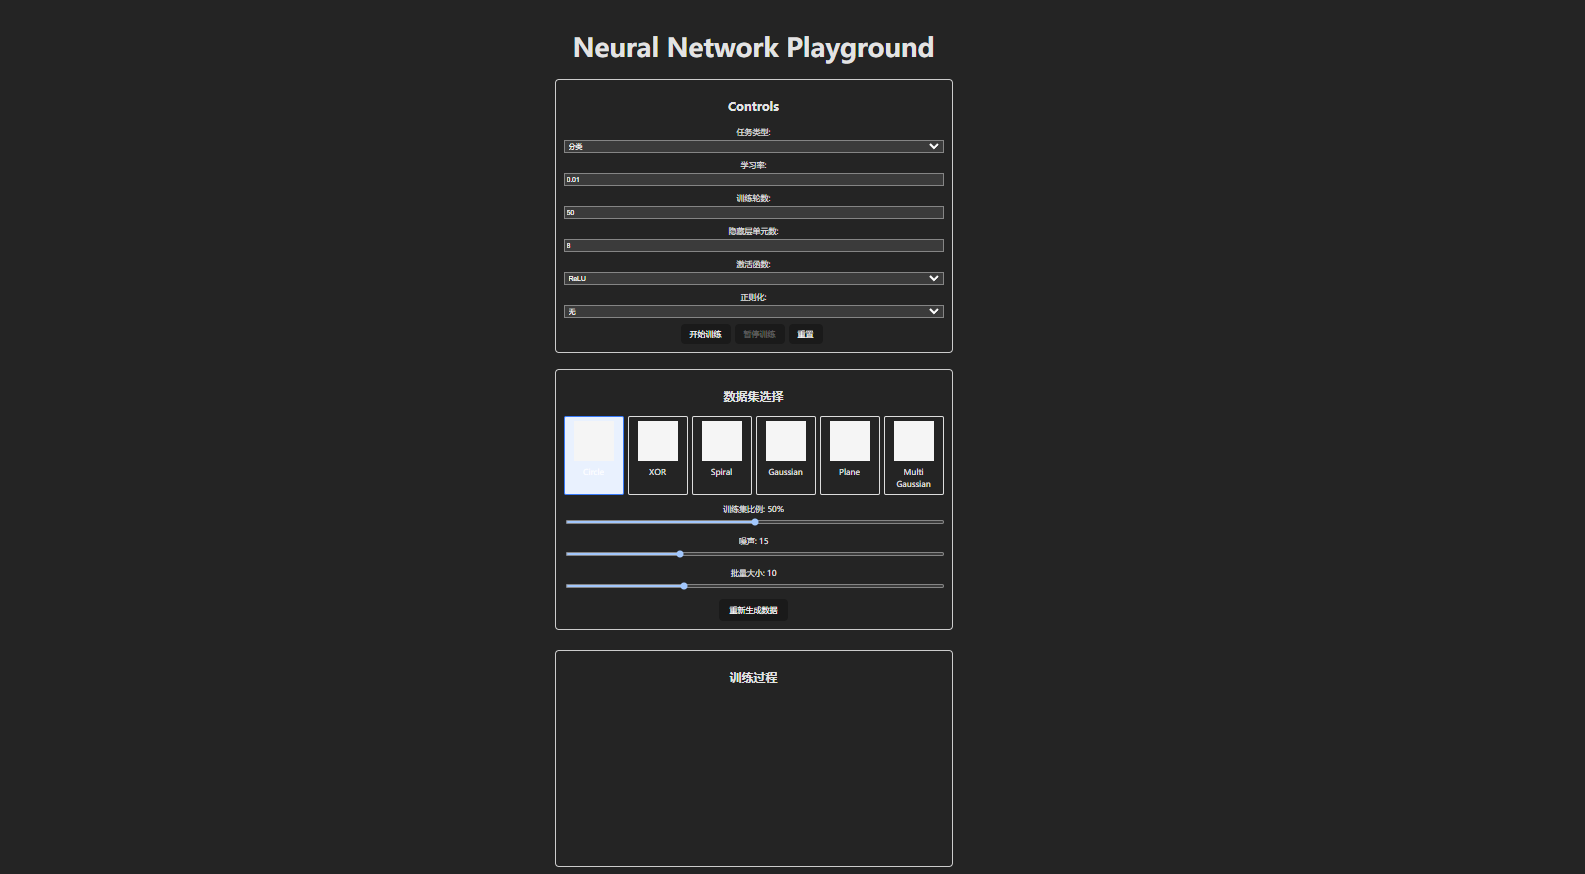
\includegraphics[width=0.8\linewidth]{image/5/2.png}
  \caption{案例总体介绍}
  \label{fig:my_label}
\end{figure}
















\section{总结}

通过本章对线性回归和逻辑回归模型学习，以及实际感受参数的调整对模型性能的影响，我们能够更加深刻地理解如何使用一个人工智能模型与参数调整对模型性能的重要影响，让读者能够对人工智能有一个更直观更全面的认识。

在5.1节中，我们从线性回归和逻辑回归模型入手，向读者回顾两种模型的发展历史、优势、局限性以及实际应用等。我们不难发现，即使是两种不同类型的模型，也可能能执行相同类型的实际任务，例如，线性回归和逻辑回归都能被运用到预测任务中。尽管实际性能可能会有所差异。因此，我们需要根据任务的实际需求选择合适的模型，有时甚至要结合多个模型。

在5.2节中，我们聚焦于模型的参数。虽然每一个模型所需要调整或得到的参数有所不同，但有一部分参数在几乎所有人工智能模型中都有应用。我们通过“烘焙慕斯蛋糕”的过程，向读者介绍模型中一些最常见的参数，以及简单讨论了参数的不同对模型性能的实际影响。

在5.3节中，我们从案例实际出发，引领读者直观地理解模型的运行过程以及模型参数的调整对于实际性能的影响，并简单阐述如何调整参数，来寻找模型最优的参数组合。

综上所述，本章内容从实际出发，以线性回归和逻辑回归模型为例，向读者详细介绍两种模型，并结合实际案例，让读者对参数调整对模型性能的影响有了直观的体会，进一步加深了读者对人工智能模型的理解。

\section{第五章习题}

\textbf{一、选择题}

\begin{enumerate}
   \item \textbf{下列哪一项不属于人工智能模型的参数？}
  \begin{enumerate}[A.]
    \item 学习率
    \item 迭代次数
    \item 输出结果
    \item 批量大小
  \end{enumerate}

  \textbf{参考答案：} C

  \item \textbf{下列哪一项不属于线性回归模型的优势？}
  \begin{enumerate}[A.]
    \item 简单易懂
    \item 非线性关系拟合能力强
    \item 灵活性
    \item 可解释性
  \end{enumerate}

  \textbf{参考答案：} B
  \end{enumerate}

